\section{Конструкторский раздел}

\subsection{Требование к ПО}

Необходимо реализовать загружаемый модуль ядра, считывать перемещение пальцев по тачпаду и выполнять заданные действия системы. Действия необходимо поместить в файл ФС \texttt{proc}.

\subsection{IDEF0}

На рисунке \ref{fig:idef} изображена диаграмма IDEF0 требуемой задачи.

\begin{figure}[h!btp]
	\centering
	\includegraphics[width=0.9\textwidth]{inc/idef.pdf}
	\caption{Диаграмма IDEF0}
	\label{fig:idef}	
\end{figure}

\subsection{Алгоритм работы обработчика}

На рисунке \ref{fig:alg} представлен алгоритм работы обработчика.

\begin{figure}[H]
	\centering
	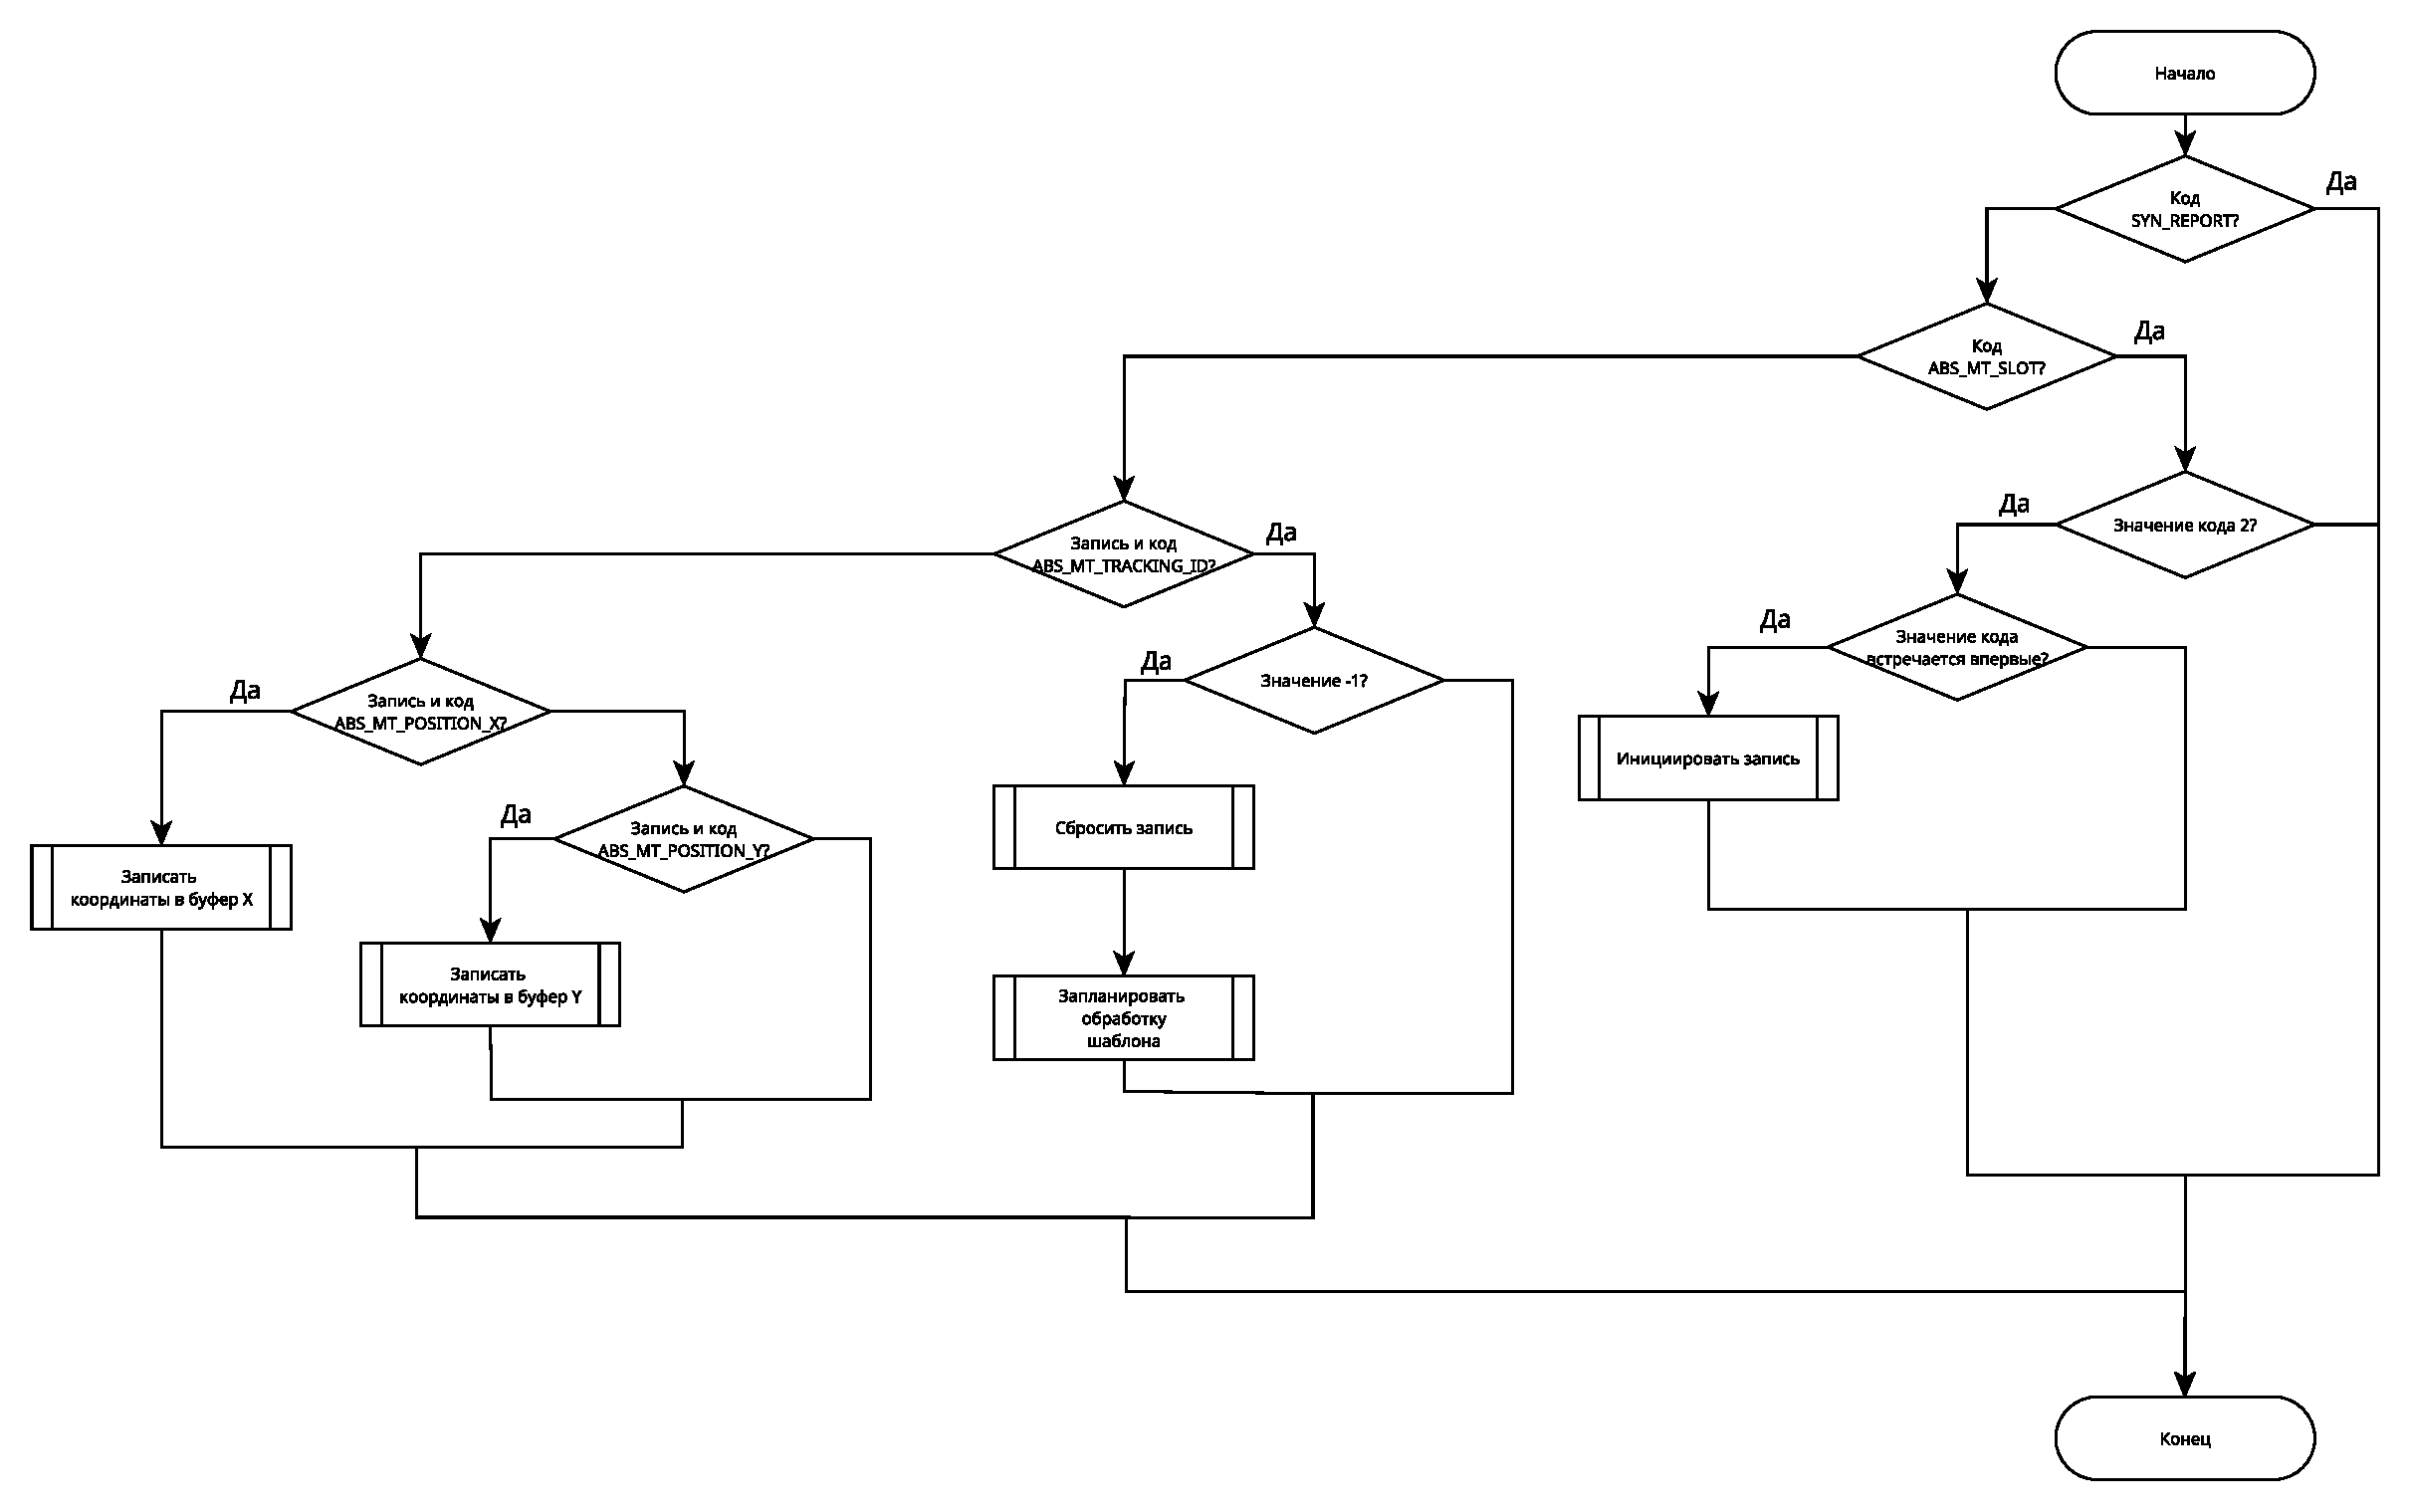
\includegraphics[width=0.65\textwidth]{inc/alg.pdf}
	\caption{Алгоритм работы обработчика}
	\label{fig:alg}
\end{figure}

\subsection{Структура ПО}

На рисунке \ref{fig:arch} представлена структура конечного ПО.

\begin{figure}[H]
	\centering
	\includegraphics[width=0.9\textwidth]{inc/arch.pdf}
	\caption{Структура ПО}
	\label{fig:arch}
\end{figure}

\clearpage
